% *************** Front matter ***************

% ***************************************************
% You should specify the contents of title page here
% Then you can specify dedication page or disable it
% ***************************************************

% *************** Title page ***************
\pagestyle{empty}
% \sffamily
% 
% \noindent
% \begin{center}
%     \Large
%     Département de Mathématiques et Applications,\\
%     \'Ecole Normale Supérieure, Paris.	
% \end{center}
% 
% \vfill\vfill
% \begin{center}
%     \large
%     Thèse en vue d'obtenir le grade de \\
%     Docteur de l'\'Ecole Polytechnique,\\
%    spécialité Mathématiques Appliquées.\\
% \end{center}
% 
% \vfill
% \begin{center}
%     \Huge\bfseries
%      Modélisation de l'électro-localisation active \\
%      chez les poissons faiblement électriques.
% \end{center}
% 
% 
% \vfill
% \begin{center}
%     \huge\bfseries
%     Thomas Boulier
% \end{center}
% 
% \vfill\vfill\vfill
% \begin{center}
%     \Large
%     Directeurs de thèse~:\\
%     Habib Ammari\\
%     Josselin Garnier
% \end{center}
% 
% \vfill
% \begin{center}
% \large
%     Paris, 2013
% \end{center}

% \begin{titlepage}

  
\includegraphics[height=3cm]{logoX.eps}
  \hfill
  
\includegraphics[height=3cm]{logoENS.eps}	
  \vskip 1cm
	\begin{center}
	\Large{\textbf{TH\`ESE}}\\
	\vskip 0.2cm
	%\normalsize
	Pr\' esent\' ee pour obtenir le grade de\\
	DOCTEUR DE L'\' ECOLE POLYTECHNIQUE\\
	\textbf{Sp\' ecialit\' e : Math\' ematiques Appliqu\' ees}\\
	par\\	
	\textbf{M. Thomas BOULIER}
	\vskip 1.5cm
	
	\centering {\huge\textbf{Modélisation de l'électro-localisation active \\
     chez les poissons faiblement électriques.}}
	\vskip 0.3cm
	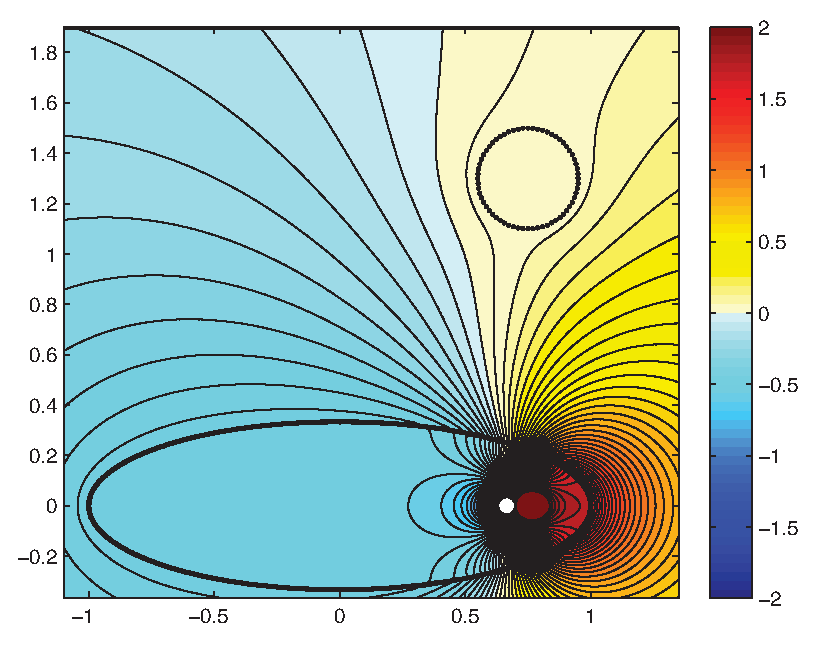
\includegraphics[height=5cm]{poisson_anomaly.eps}
	\vskip 0.2cm
	
	 Soutenue le 21 juin 2013 devant le jury compos\' e de:\\
\begin{tabular}{ll}
M.\ Habib AMMARI & \textsl{Directeur de Th\`ese}\\
M.\ Josselin GARNIER & \textsl{Directeur de Th\`ese}\\
M.\ Oscar BRUNO & \textsl{Rapporteur}\\
M.\ Jin Keun SEO & \textsl{Rapporteur}\\
M.\ Hongkai ZHAO & \textsl{Rapporteur}\\
M.\ Grégoire ALLAIRE & \textsl{Examinateur}\\
M.\ Frédéric BOYER & \textsl{Examinateur}\\
M.\ Stéphane MALLAT & \textsl{Examinateur}\\
Mme\ Liliana BORCEA & \textsl{Invitée}\\
\end{tabular}	

\end{center}
% \end{titlepage}

\cleardoublepage

% *************** Dedication ***************
\vspace*{\fill}
{\hfill\sffamily\itshape \`A ma famille.}
\cleardoublepage

\rmfamily
\normalfont

% *************** Citation ***************


\begin{changemargin}{6cm}{-3cm}
{\sffamily
\itshape
\begin{quote}
Je chante les héros dont Esope est le père,  \\
Troupe de qui l'histoire, encor que mensongère, \\ 
Contient des vérités qui servent de leçons. \\
Tout parle en mon ouvrage, et même les poissons: \\
Ce qu'ils disent s'adresse à tous tant que nous sommes; \\
Je me sers d'animaux pour instruire les hommes.\\
\end{quote}
}
\sffamily
\begin{flushleft}
Jean de La Fontaine, Fables.\\
A Monseigneur le Dauphin,
Livre I - Fable 0.
\end{flushleft}
\end{changemargin}

\vspace*{\fill}

\cleardoublepage

\rmfamily
\normalfont

% *************** Table of contents ***************
\pagenumbering{roman}
\pagestyle{headings}
\tableofcontents

% *************** End of front matter ***************
